\chapter{DESENVOLVIMENTO DO SISTEMA}
\label{cap:sistema}	

Neste capítulo são abordadas as fases de desenvolvimento do software.

\section{Especificação de requisitos}


O módulo proposto visa satisfazer as necessidades do professor, quanto a utilização dos recursos do diário virtual. Isso impossibilita o compartilhamento de informações necessárias ao professor, como a lista de alunos por exemplo, que deveria ser fornecida por outro módulo (secretaria). Logo, a inserção desses dados fazem parte dos requisitos do sistema atual. Na Tabela \ref{tab:reqfuncionais} são descritos os requisitos funcionais levantados para o modo professor.


\begin{table}[h]
	
	\vspace{0.5cm}.
	\centering
	\begin{tabular}{lll}
		%coluna separa-se por &
		% \\ quebra de linha 
		% \hline para linha horizontal
		\hline	
		Identificador & Descrição \\
		\hline
		RF001 &	O software deve possibilitar adicionar um Diário \\
		RF002 &	O software deve possibilitar a visualização do Diário \\
		RF003 &	O software deve possibilitar a exclusão do Diário \\
		
		RF004 &	O software deve possibilitar a visualização dos Alunos\\
		RF005 &	O software deve possibilitar adicionar um novo Aluno\\
		RF006 &	O software deve possibilitar excluir Aluno\\
		RF007 &	O software deve possibilitar alterar Aluno\\
		
		RF008 &	O software deve possibilitar a visualização das Aulas\\
		RF009 &	O software deve possibilitar adicionar uma nova Aula\\
		RF010 &	O software deve possibilitar excluir Aula\\
		RF011 &	O software deve possibilitar alterar Aula\\
		
		RF012 &	O software deve possibilitar a visualização das Avaliaçãoes\\
		RF013 &	O software deve possibilitar adicionar uma nova Avaliação\\
		RF014 &	O software deve possibilitar excluir Avaliação\\
		RF015 &	O software deve possibilitar alterar Avaliação \\
		
		\hline
	\end{tabular}
	\caption{Requisitos funcionais}
	\label{tab:reqfuncionais}
\end{table}

Estes, foram traduzidos para um diagrama de caso de uso, que por sua vez tem a função de documentar o que o sistema faz, no ponto de vista do usuário. Ele pode ser observado na Figura \ref{fig:UseCaseDiagram0}; o professor, que é o único usuário do módulo, consegue realizar tarefas (casos de uso) no sistema, para cada diário que ele possuir.

\begin{figure}[!htb]
	\centering
	\caption{Diagrama de caso de uso} %legenda
	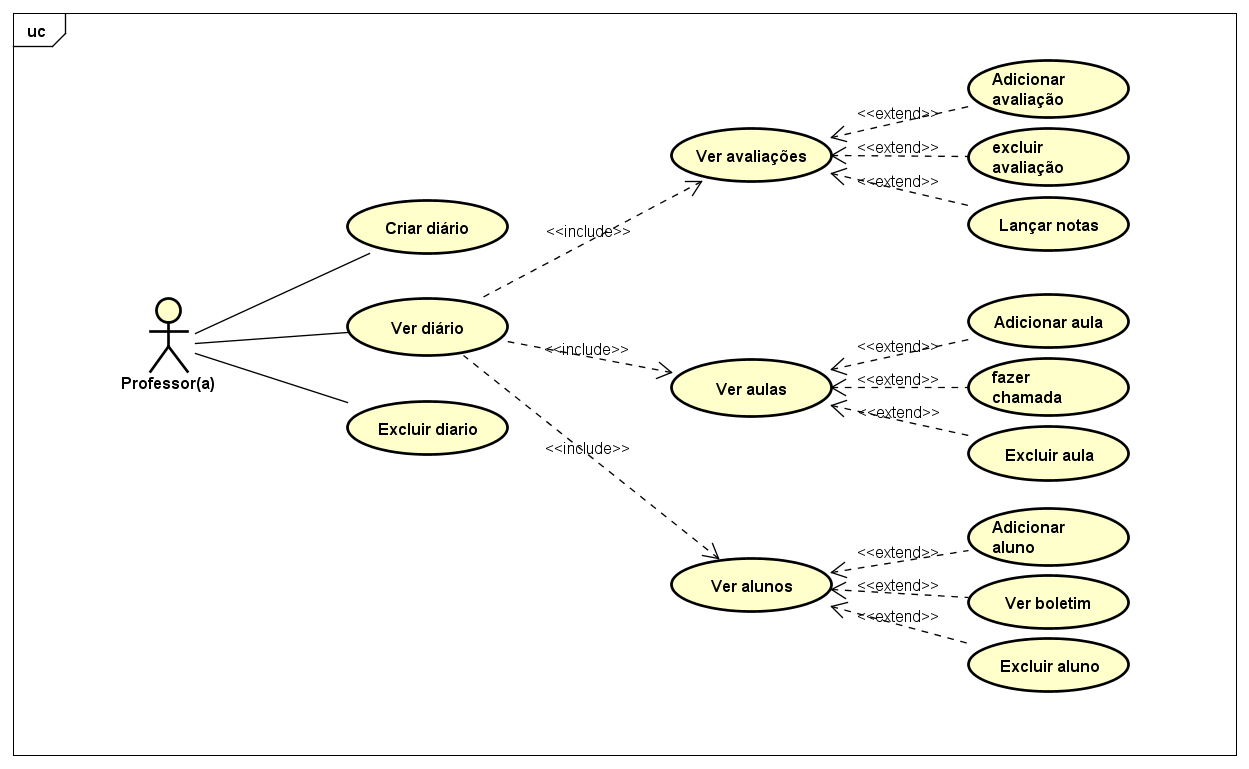
\includegraphics[scale=0.4]{UseCaseDiagram0}\\  % o 0.9 indica 90% do tamanho original
	% pdfLaTeX aceita figuras no formato PNG, JPG ou PDF
	% figuras vetoriais podem ser exportadas para eps e depois convertidas para pdf usando epstopdf
	{\small } %Fonte da imagem
	\label{fig:UseCaseDiagram0} %rotulo para refencia
\end{figure}




\section{Projeto}


O professor desempenha tarefas importantes com o uso do diário. São elas:

\begin{itemize}
	\item Efetuar o registro da aula, informando a data e um resumo geral específico sobre o conteúdo lecionado nesse dia.
	
	\item Registrar também qualquer ocorrência ou fato relevante que aconteça em sala de aula
	
	\item Realizar a chamada colocando "presença" ou "falta" para cada aluno matriculado na matéria referente a chamada.
	
	\item Transcrever as atividades avaliativas e informar o valor atribuído a cada uma delas, bem como a nota obtida por cada aluno nestas atividades.
	
	\item Fechar as notas de cada aluno ao final do período escolar, preenchendo a taleta (relatório).
	
	
\end{itemize}

Tais tarefas foram transcritas ao ambiente de desenvolvimento em formas de adaptações na produção da interface. 

O módulo permite que cada professor acesse o conteúdo de seus diários. Para isso, é preciso efetuar \textit{login} com \textit{e-mail} e senha, possibilitando a criação de um novo cadastro, caso ainda não possua. Dentro de cada diário estão disponíveis cadastro e acesso à alunos, avaliações e aulas. 



\subsection{Estruturação do banco de dados}

Após a definição dos principais requisitos do sistema e suas funcionalidades, foi estruturado uma base de dados para armazenar as informações necessárias para o funcionamento do módulo. Para isso, optou-se pelo modelo relacional, que possibilita criar entidades e o relacionamento entre elas.

As entidades modeladas (tabelas) representam as principais estruturas de dados necessárias para implementação das funcionalidades do sistema. São elas nomeadas de: Professor, Diário, Aluno, Avaliação, Nota, Chamada, Aula, PeriodoDeRegime e Turma. Tais nomes foram adotados,  sugestivamente, como abstração dos objetos do mundo real para facilitar o entendimento. Assim, podemos dizer por exemplo que, nesse sistema, dadas as necessidades, o Professor(representado pela tabela professor) possui atributos (dados) "nome, e-mail, senha e uma imagem de perfil".

A estrutura final das entidades e do relacionamento entre elas, é apresentado na Figura \ref{fig:relacional}. O script SQL (\textit{Structured Query Language}, ou Linguagem de Consulta Estruturada) exportado, é utilizado pelo servidor para criação e disponibilização ao banco de dados para uso na aplicação.  

\begin{figure}[!htb]
	\centering
	
	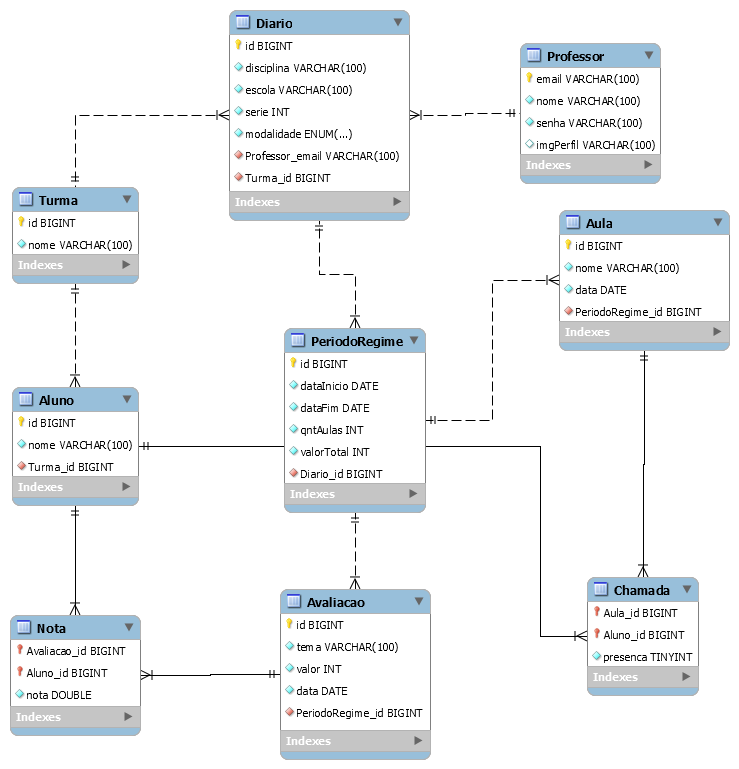
\includegraphics[scale=0.6]{relacional}\\  % o 
	\caption{Modelo relacional do banco de dados} %legenda
	{\small } %Fonte da imagem
	\label{fig:relacional} %rotulo para refencia
\end{figure}

\section{Implementação}


Para desenvolvimento do software, adotou-se o uso da arquitetura \textit{Model-view-controller} - MVC. Tal arquitetura propõe que seja feita a separação da representação da informação (dados), da interação do usuário (interface). A arquitetura da implementação do Diário de Classe encontra-se estruturada em três diretórios: \textit{Model}, \textit{View} e \textit{Controller}. Tal divisão com seus respectivos arquivos são mostrados na Figura \ref{fig:controller-model} e Figura \ref{fig:view}.

\begin{figure}[!htb]
	\centering
	
	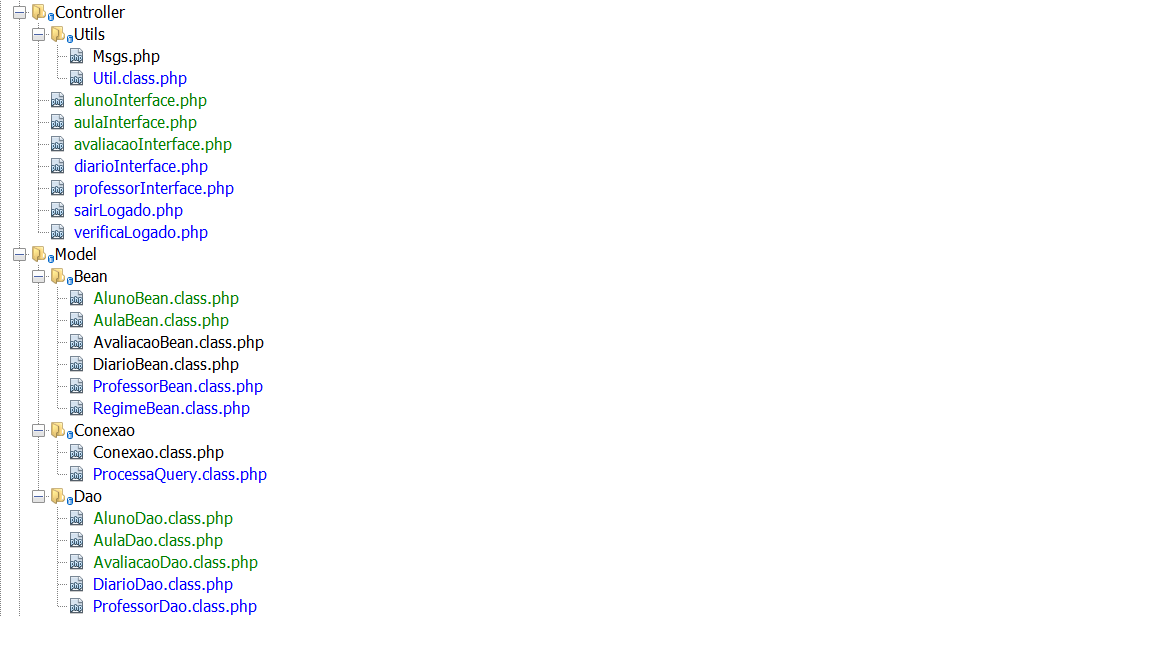
\includegraphics[scale=1.0]{controller-model}\\  % o 0.9 indica 90% do tamanho original
	% pdfLaTeX aceita figuras no formato PNG, JPG ou PDF
	% figuras vetoriais podem ser exportadas para eps e depois convertidas para pdf usando epstopdf
	\caption{Divisão dos diretórios - controller e model} %legenda
	{\small } %Fonte da imagem
	\label{fig:controller-model} %rotulo para refencia
\end{figure}

\begin{figure}[!htb]
	\centering	
	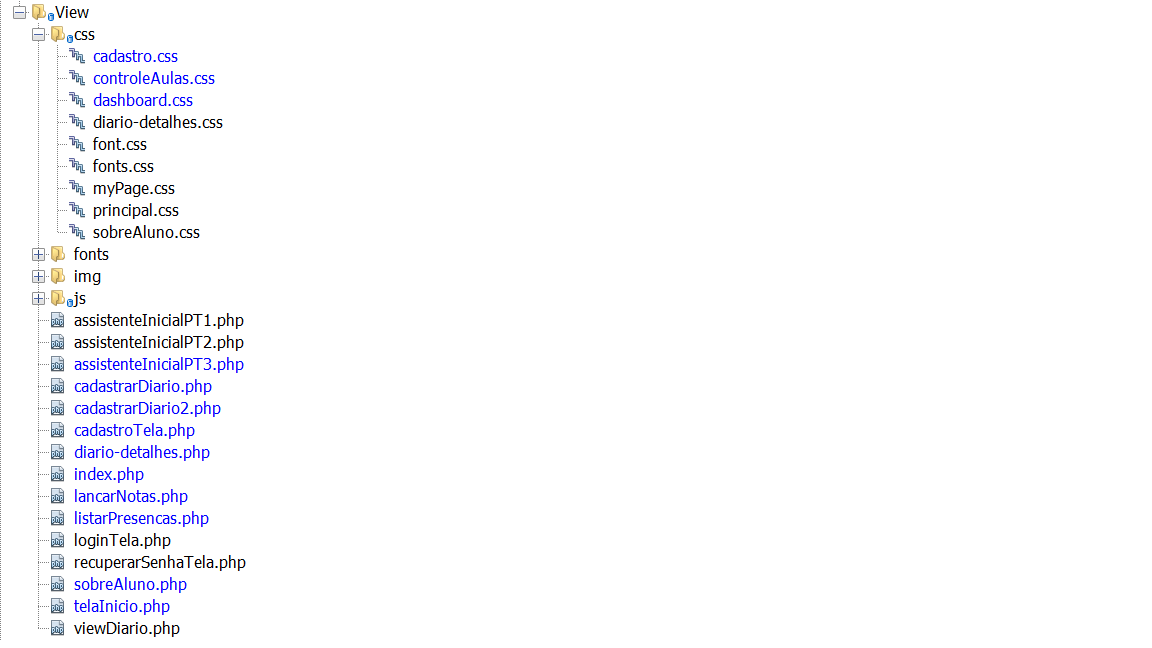
\includegraphics[scale=0.9]{view}\\  % o 0.9 
	\caption{Divisão dos diretórios - view} %legenda
	{\small } %Fonte da imagem
	\label{fig:view} %rotulo para refencia
\end{figure}

No \textit{Model}, estão os objetos e seus respectivos \textit{gets} e \textit{sets}, bem como as classes que estabelecem conexão ao banco de dados e as classes de acesso a dados (DAO - \textit{Date Acess Object}). Essa estruturação permite que quando ocorra mudança nos dados de qualquer objeto, seja fácil a notificação para classes que exercem controle sobre esses dados e o repasse para as classes responsáveis às "visões" do usuários.

A interface se localiza no \textit{View}. Ali estão todos os códigos em HTML, CSS e JS responsáveis pela renderização do conteúdo que interage com o usuário, imagens e fontes tipográficas. Por último, mas não menos importante, temos o diretório \textit{Controller}, onde ficam as principais tarefas e requisições, controladas por comandos em PHP. Em exemplo: toda ação de cadastro de um "professor" é captada por um campo na interface \textit{view} e transmitido para o \textit{controller} "professorInterface.php" que é responsavel por analisar os comandos e direcinar o caminho de cada tipo de ação para sua tarefa, esperar uma resposta e executar uma ação de retorno com essa resposta para a \textit{view}.

Ao entrar no sistema, o usuário se depara com duas opções: se cadastrar ou \textit{logar} no sistema. Na primeira, o usuário insere dados de \textit{e-mail}, senha, nome e imagem de perfil(opcional). Após prosseguir, na \textit{view} os dados são encaminhados para interfaceProfessor.php que chama o \textit{bean} responsável por registrar os dados. Esses dados são devolvidos a ele, que solicita a classe DAO (\textit{Data Access Object}) que armazene os dados no banco. As Figuras \ref{fig:loginoucadastro}, \ref{fig:cadastroview},
 \ref{fig:cadastroview1},
 \ref{fig:cadastroview2},
 \ref{fig:cadastroview3},
 \ref{fig:cadastroview4}, e
 \ref{fig:cadastroview5} respectivamente, mostram os arquivos com o fluxo de dados descrito.
 


\begin{figure}[!htb]
	\centering
	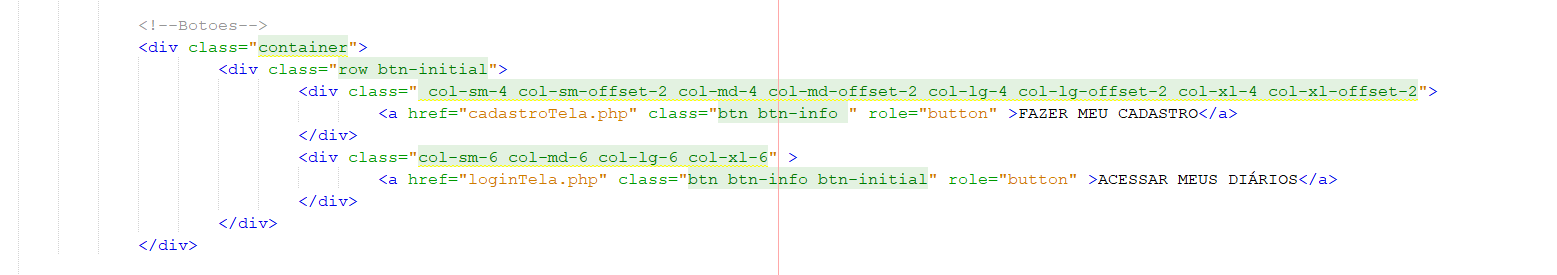
\includegraphics[width=0.9\linewidth]{loginOuCadastro}
	\caption{Arquivo "index.php"}
	\label{fig:loginoucadastro}
\end{figure}

\begin{figure}[!htb]
	\centering
	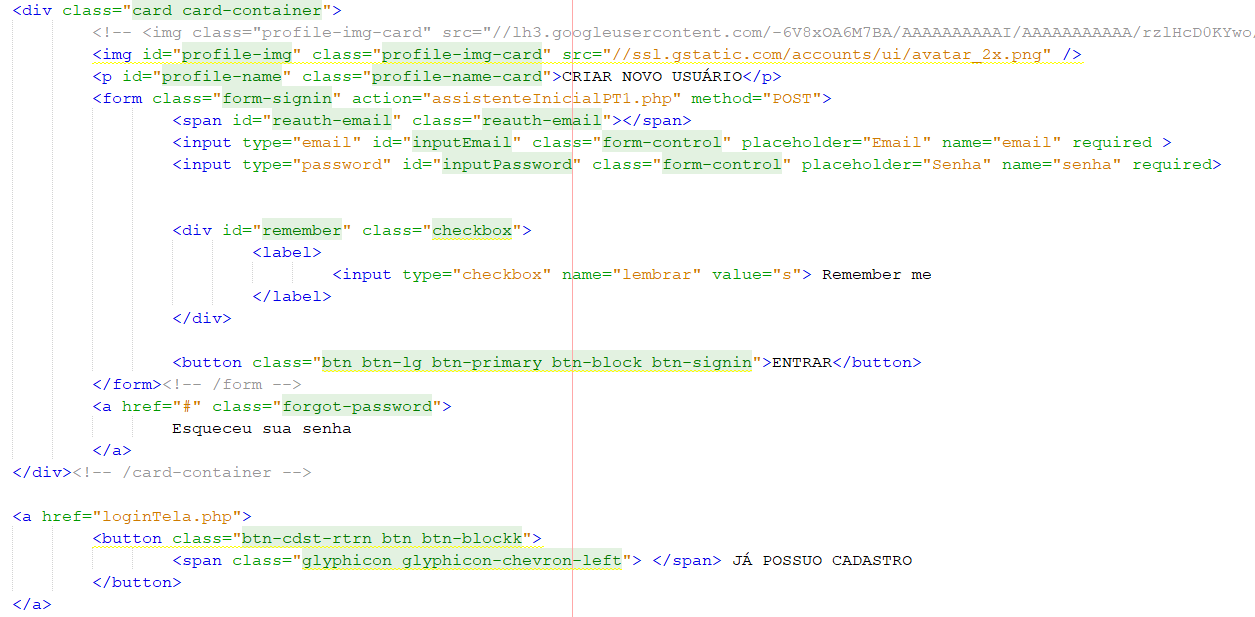
\includegraphics[width=0.9\linewidth]{cadastroView}
	\caption{Arquivo "cadastroTela.php" }
	\label{fig:cadastroview}
\end{figure}

\begin{figure}[!htb]
	\centering
	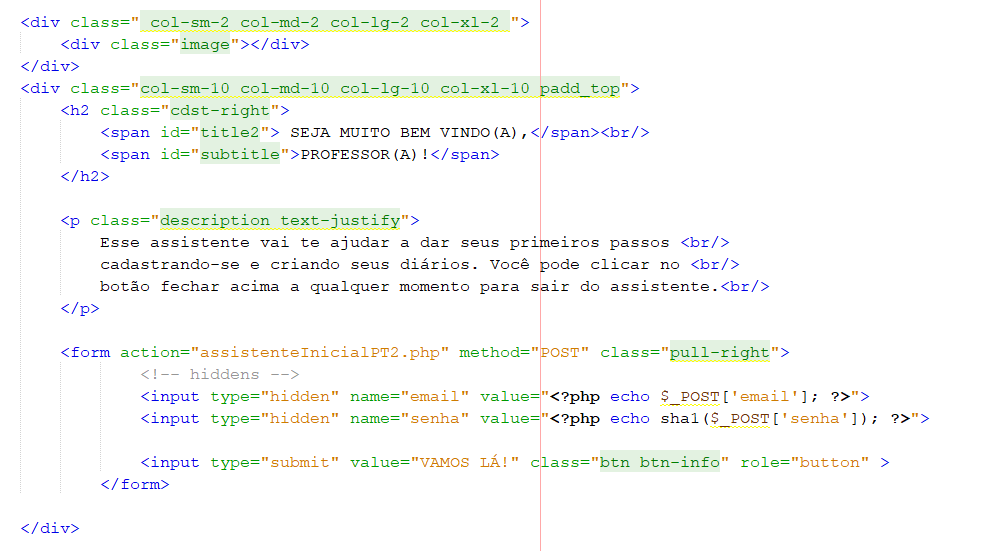
\includegraphics[width=0.9\linewidth]{cadastroView1}
	\caption{Arquivo "assistenteInicialPT1.php"}
	\label{fig:cadastroview1}
\end{figure}


\begin{figure}[!htb]
	\centering
	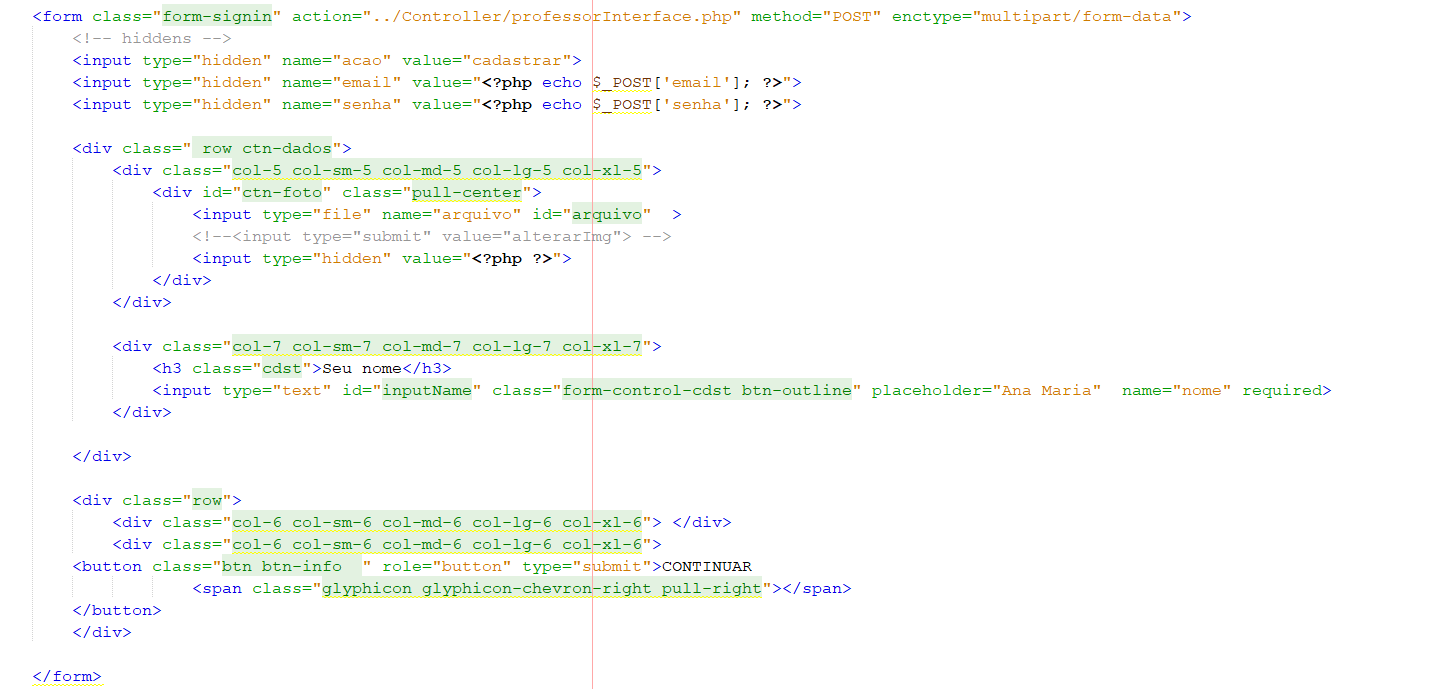
\includegraphics[width=0.9\linewidth]{cadastroView2}
	\caption{Arquivo "assistenteInicialPT2.php"}
	\label{fig:cadastroview2}
\end{figure}

\begin{figure}[!htb]
	\centering
	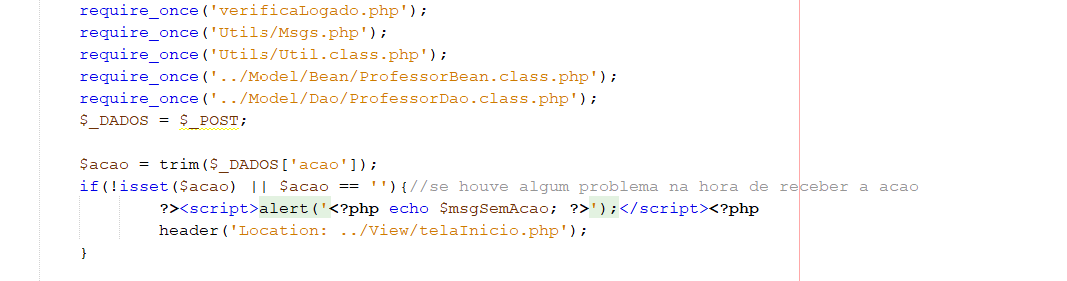
\includegraphics[width=0.9\linewidth]{cadastroView3}
	\caption{Arquivo "assistenteInicialPT3.php"}
	\label{fig:cadastroview3}
\end{figure}

\begin{figure}[!htb]
	\centering
	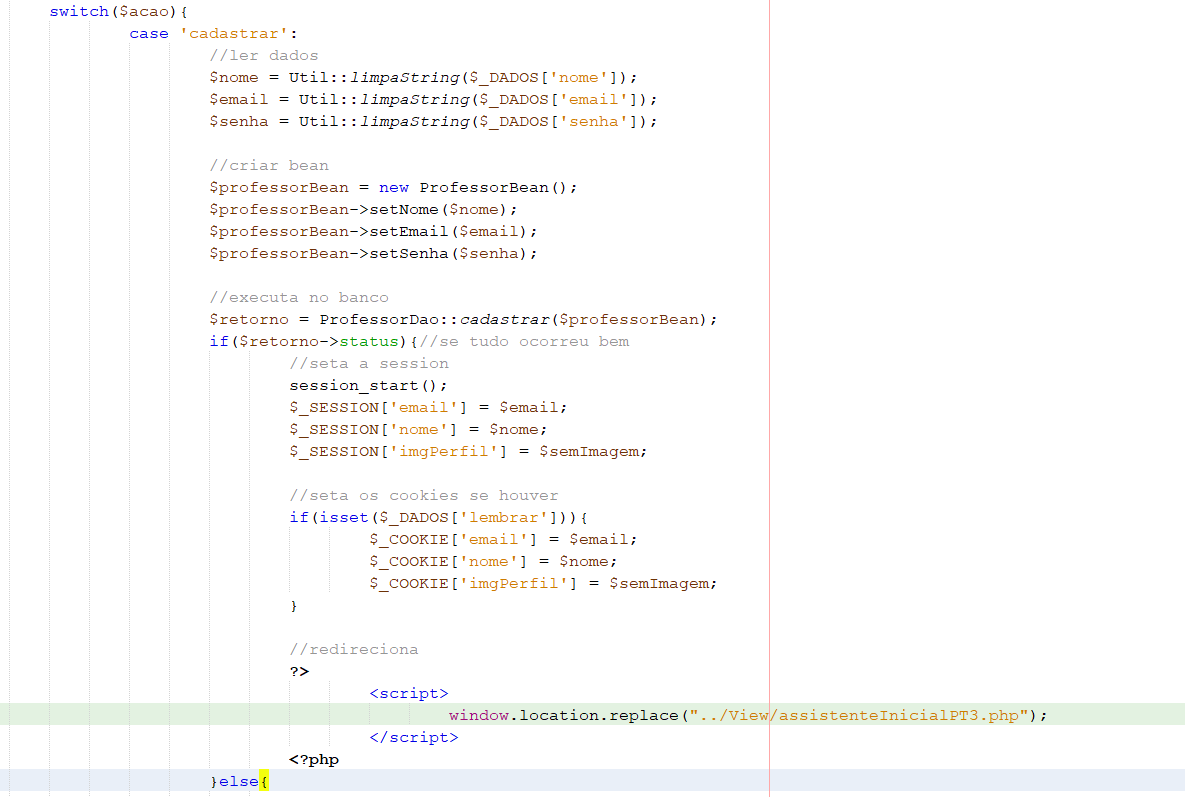
\includegraphics[width=0.9\linewidth]{cadastroView4}
	\caption{Arquivo "professorInterface.php"}
	\label{fig:cadastroview4}
\end{figure}

\begin{figure}[!htb]
	\centering
	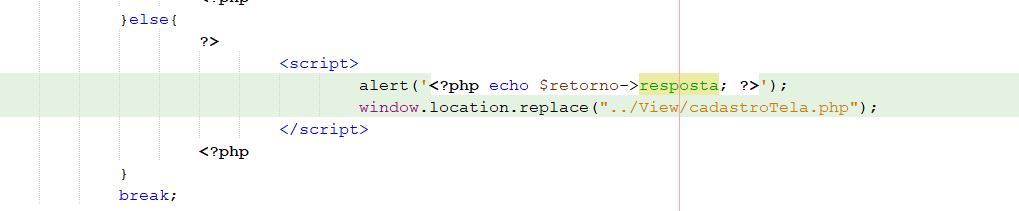
\includegraphics[width=0.9\linewidth]{cadastroView5}
	\caption{Arquivo "professorInterface.php"  - continuação da figura \ref{fig:cadastroview4}}
	\label{fig:cadastroview5}
\end{figure}

As estrutura das classes utilizadas no cadastro acima exemplificado, são mostradas nas figuras \ref{fig:cadastroview6} e \ref{fig:cadastroview7}.

\begin{figure}
	\centering
	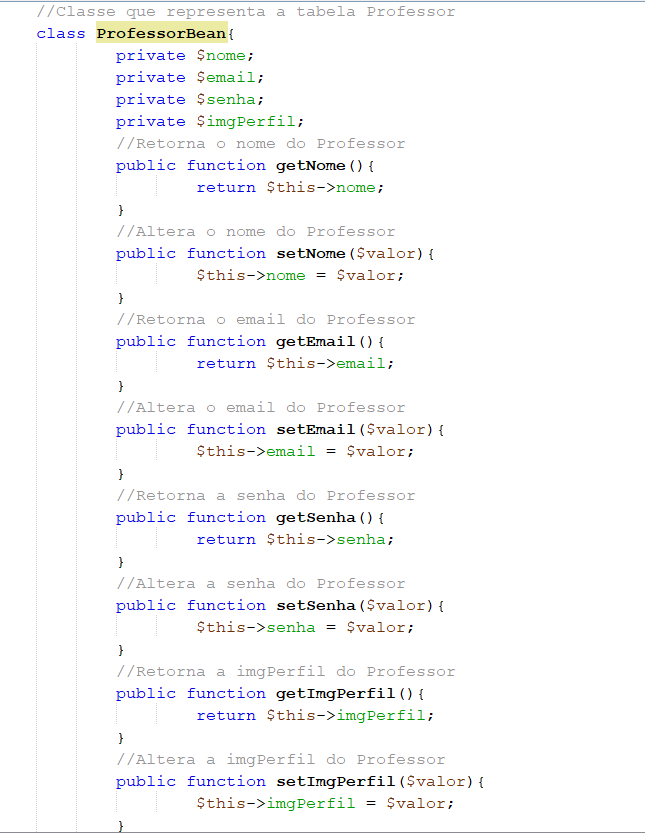
\includegraphics[width=0.9\linewidth]{cadastroView6}
	\caption{Classe "ProfessorBean.class.php"}
	\label{fig:cadastroview6}
\end{figure}

\begin{figure}
	\centering
	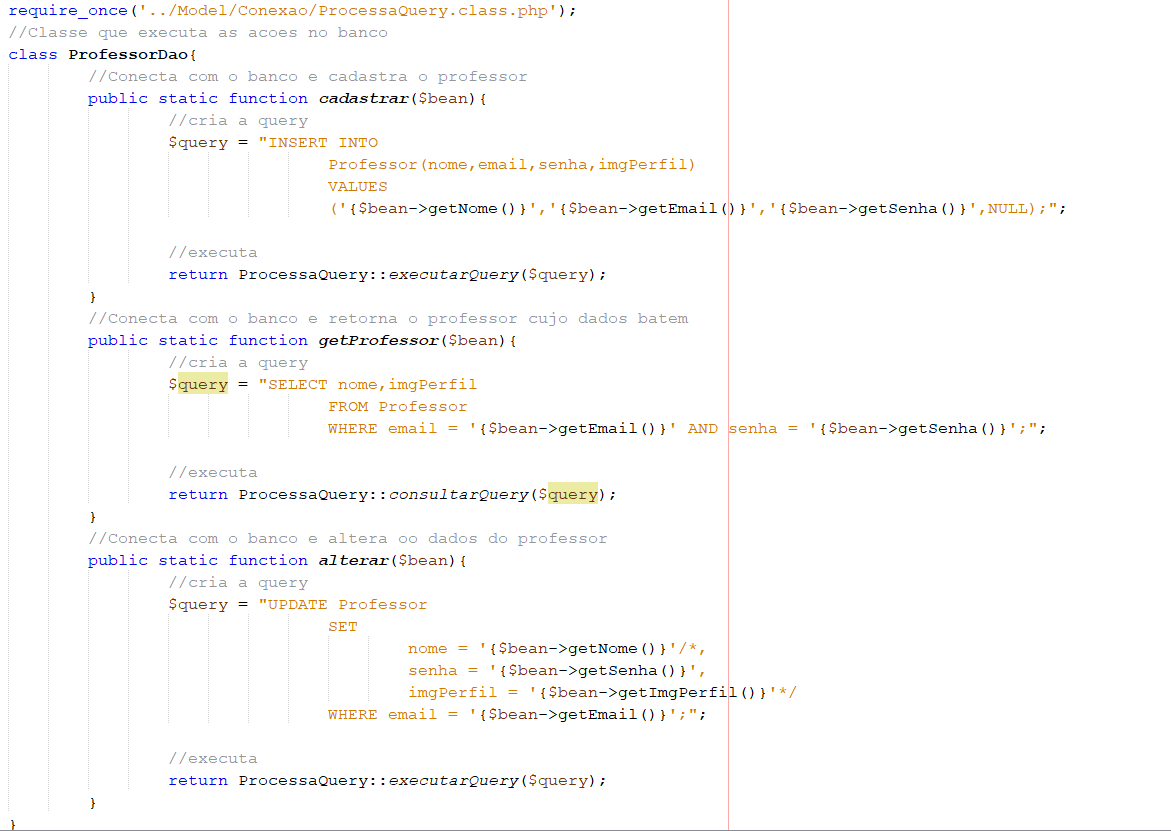
\includegraphics[width=0.9\linewidth]{cadastroView7}
	\caption{Classe "ProfessorDao.php"}
	\label{fig:cadastroview7}
\end{figure}




\section{Testes}

Os testes feitos na aplicação, são baseados no conceito de "teste de caixa preta". Tal tipo de teste (também chamado de funcional ou de validação), tem por objetivo avaliar o comportamento externo de cada componente, utilizando a saída obtida por uma entrada, com o resultado esperado.

Os testes foram feitos durante a fase de desenvolvimento para testar fluxo de dados, inspecionar condições, variáveis e outros, através da utilização da interface gráfica para validação.

